\documentclass[12pt]{article} 
\usepackage{natbib}
\usepackage{a4wide}
\usepackage{lineno}
\usepackage{cancel}

\newif\ifbuch
\global\buchtrue
\global\buchfalse

\newif\ifdetail
\global\detailfalse
%\global\detailtrue

\usepackage{color}
\usepackage[pdftex]{graphicx}
\usepackage[pdftex,colorlinks,
                citecolor=darkgreen,linkcolor=darkblue,urlcolor=darkblue]{hyperref}
\definecolor{darkgreen}{rgb}{0.1,0.4,0.1}
\definecolor{darkblue}{rgb}{0.1,0.1,0.3}

\usepackage{amssymb}
\def\bem#1{\colorbox{green}{\em #1}}


\newcommand{\beq}  { \begin{eqnarray} }
\newcommand{\eeq}  { \end{eqnarray}}
\newcommand{\beeq}  { \begin{eqnarray*} }
\newcommand{\eeeq}  { \end{eqnarray*}}
\newcommand{\eq }  [1]{Eq.~(\ref{#1})}  % Eq. (#1)
\newcommand{\sect}  [1]{Sec.~(\ref{#1})}  % Eq. (#1)
\newcommand{\fig}  [1]{Fig.~\ref{#1}}   % Fig. #1
\renewcommand{\v}[1]{{\mbox{\boldmath$ #1 $}}}  % Vektor durch Fettdruck
\newcommand{\m}    [1]{{\bf  #1 }}              % Matrix in sans serif
\newcommand{\gz}[1] {{{d #1} \over {dz}}}
\newcommand{\pt}[1]{{\partial_t #1}}
\newcommand{\ptt}[1]{{{\partial^2 #1} \over {\partial t^2}}}
\newcommand{\pttx}[1]{{{\partial^3 #1} \over {\partial t^2 \partial x}}}
\newcommand{\ptty}[1]{{{\partial^3 #1} \over {\partial t^2 \partial y}}}
\newcommand{\pttt}[1]{{{\partial^3 #1} \over {\partial t^3}}}
\newcommand{\ptx}[1]{{{\partial^2 #1} \over {\partial t \partial x}}}
\newcommand{\pty}[1]{{{\partial^2 #1} \over {\partial t \partial y}}}
\newcommand{\pz}[1]{{\partial_z #1}}
\newcommand{\pzz}[1]{{\partial_{zz} #1}}
\newcommand{\px}[1]{{\partial_x #1}}
\newcommand{\py}[1]{{\partial_y #1}}
\newcommand{\pxi}[1]{{\partial_i #1}}
\newcommand{\pxj}[1]{{\partial_j #1}}
\newcommand{\pxk}[1]{{\partial_k #1}}
\newcommand{\pb}[1]{{{\partial #1} \over {\partial b}}}
%\newcommand{\pxy}[1]{{{\partial^2 #1} \over {\partial x \partial y}}}
\newcommand{\pxy}[1]{\partial_{xy} #1}
\newcommand{\pyy}[1]{\partial_{yy} #1}
\newcommand{\pxx}[1]{\partial_{xx} #1}
\newcommand{\kx}{{\bf k} \times}
\newcommand{\dt}[1]{{{d #1} \over {d t}}}
\newcommand{\Dt}[1]{{{D #1} \over {D t}}}
\newcommand{\Div}[1]{ \nabla \cdot #1 }
\renewcommand{\div}[1]{ \nabla_{yz} \cdot #1 }
\newcommand{\Bar}[1]{ \overline{ #1} }
\newcommand{\rvec} [1]{
    \raisebox{-1.5ex}{$\stackrel{\textstyle #1}{\neg}$} }% rotierter Vektor
\newcommand{\nablq}   {\rvec\nabla}                    % rotated nabla operator
\newcommand{\Vec}[1]{\left(\begin{array}{c} #1 \end{array}\right) }
%\renewcommand{\mho}{\mathcal{W}}
\newcommand{\pn}[1]{{{\partial #1} \over {\partial n}}}
\newcommand{\pnn}[1]{{{\partial #1} \over {\partial m}}}
\newcommand{\ps}[1]{{{\partial #1} \over {\partial s}}}

\newcommand{\p}{{\partial}}
\newcommand{\vn}{{\v \nabla}}
\newcommand{\tl}{\tilde}
\newcommand{\lk}{\left(}
\newcommand{\rk}{\right)}

\begin{document} 


  \subsection*{Two-phase model}

The two-dimensional two-phase model of water and air is given by
\beq
 \p_t u  + \p_x   u u  + \p_z w u - f v &=& - (\p_x p)  /\rho
 \\
 \p_t v  + \p_x   u v  + \p_z w v + f u &=& 0
 \\
  \p_t  w  +  \p_x   u w  + \p_z w w &=& - (\p_z p)/\rho   - g 
  \\
  \p_x u + \p_z w  &=&0
  \eeq
  which holds both in water with $\rho=\rho_o$ and air with $\rho=\rho_a$,
  and 
  $\rho = c \rho_o + (1-c) \rho_a$.  %= \rho_a + c (\rho_0 - \rho_a)
 
   Solve this with two level discrete time step. Knowing $u^n$ and $w^n$ from previous time step,
  first calculate intermediate solution  $u^*$ and $w^*$ from 
  \beq
    \frac{u^*-u^n}{\Delta t} = - (\p_x   u u  + \p_z w u)_d ~,~
      \frac{w^*-w^n}{\Delta t} = -(\p_x   u w  + \p_z w w )_d - g   ~,~
  \eeq
  Then take divergence and  calculate pressure $p$ such that
   \beq
    \p_z u^*  + \p_z w^* =  - \Delta t (  \p_x (\p_x p)  /\rho + \p_z  (\p_z p)/\rho  ) 
  \eeq
 This is solved for $p$  with conjugate gradient solver with preconditioner, and so
 \beq
  u^{n+1}  = u^* - \Delta t  (\p_x p)  /\rho ~,~w^{n+1} = w^* -  \Delta t  (\p_z p)  /\rho 
 \eeq
  such that next time step $u^{n+1}$ and $w^{n+1}$ is also free of divergence.
  
  Concentration $c$ with $c=1$ in water and $c=0$ in air given by 
  \beq
  \p_t c +  \p_x   u c  + \p_z w c  = \p_z  M(c) \p_z   \mu  ~,~ 0 < c < 1 
  \eeq
  with chemical potential $\mu$ and mobility parameter $M$ given by
  \beq
   \mu =  12 c^2 - 12c  + 2~,~M_c (1- \gamma \phi^2) ~,~  \phi = 2 c-1  ~,~-1 < \phi < 1 
\eeq
\centerline{ 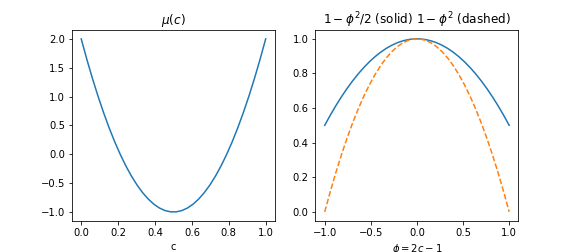
\includegraphics[width=0.9\textwidth]{mu1} }

and $M_c = 10^{-4}$ 

\section*{Discretisation}


Discretisation is on a C-grid.

\section*{Options}

The configuration is controlled in the template subroutines {\sc set\_parameter}
and {\sc initial\_conditions}. One example is provided. 

A number of switches can be set to either true or false.

\begin{tabular}{l  l  l }
 name & default & meaning \\
enable\_upwind3\_advection  & false & \\
   enable\_dst3\_advection     & false \\
 enable\_superbee\_advection & false\\
 enable\_multidim\_advection & false \\
 enable\_AB3\_time\_stepping  & false \\
enable\_particles          & false \\
 enable\_v\_velocity         & false \\
\end{tabular}

\end{document}